\section{Linearization: Correctness of Concurrent Datatypes}
\label{sec:linearization}

We want to test the concurrent total queue implementation.  But first, we need
to understand better what ``correct'' actually means in this case.  And, by
extension, we will understand correctness conditions for other concurrent
datatypes. 

We define a \emph{history} to be a sequence of calls and returns of
operations, corresponding to threads operating on the datatype.
Informally, a history is correct if:
%
\begin{itemize}
\item Operation executions take place (apparently) in a one-at-a-time
  way, without interference between different executions.

\item The point at which each operation execution takes effect is between the
time the invocation was invoked and when it returns; we call this point
the \emph{linearization point}.

\item The values returned by operation executions should be the same as for a
sequential queue (when the executions are performed in the same order).
\end{itemize}
%
The correctness condition for other concurrent datatypes is the same, except
with the sequential queue in the third item replaced by a corresponding
sequential datatype.

This property is called \emph{linearization}~\cite{herlihy-wing}.  It is an
attractive property, because it matches most programmers' mental models of how
such a concurrent datatype should behave.

We will give a more formal definition of linearization shortly.  But first, we
give some examples.  

Figure~\ref{fig:linearization} gives four timelines depicting histories.  In
each timeline, time goes from left to right.  Each row is labelled with the
identity of a thread (e.g.~$t_0$).  Each horizontal line represents the
execution of an operation, with the endpoints of the line representing the
call of the operation and its return, respectively; the line is labelled with
the name of the operation, its parameters, and the value returned, although we
omit the latter for operations, like |enqueue|, that return the trivial |Unit|
type.

%%%%%

\begin{figure}
\def\X{node{\scalastyle X};}
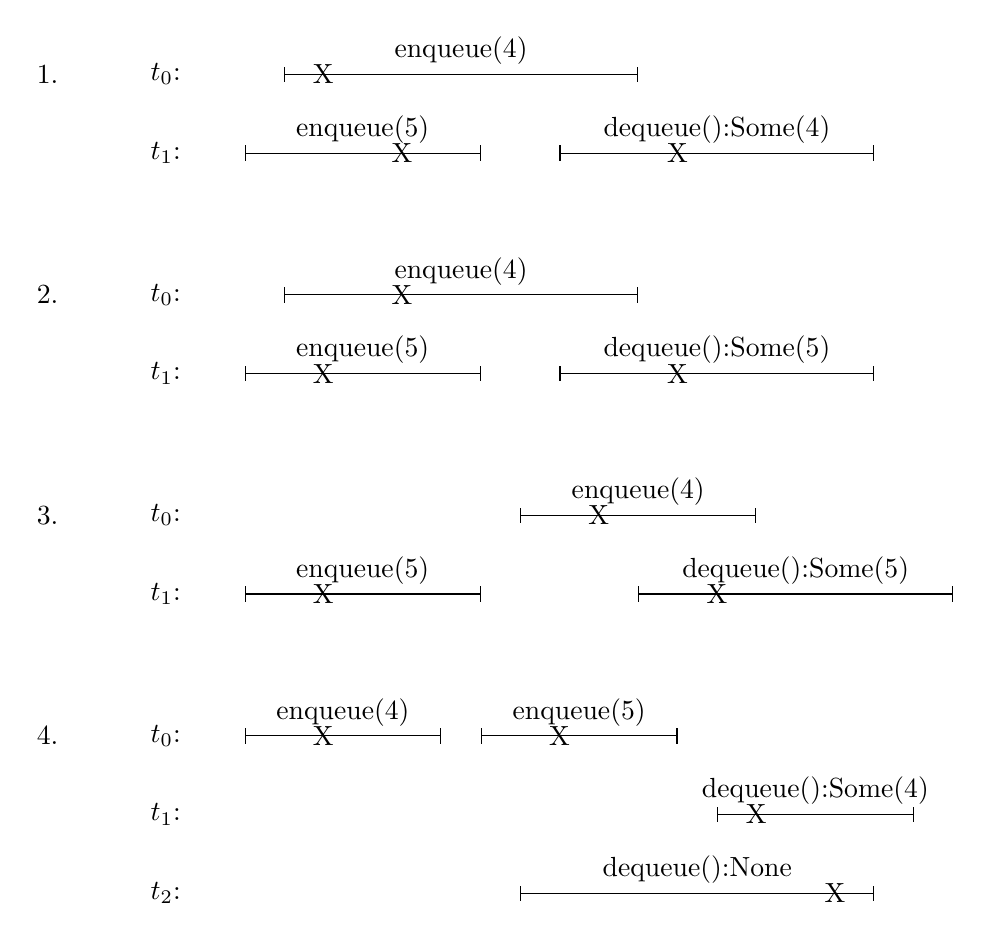
\begin{tikzpicture}[scale=1.0]
\draw (-1.5,0) node{1.};
\draw (0,0) node {$t_0$:}; 
\draw[|-|] (1.5,0) -- node[above] {\scalashape enqueue(4)} (6,0);
\draw(2,0) \X;
\draw (0,-1) node {$t_1$:}; 
\draw[|-|] (1,-1) -- node[above] {\scalashape enqueue(5)} (4,-1);
\draw(3,-1) \X;
\draw[|-|] (5,-1) -- node[above] {\scalashape dequeue():Some(4)} (9,-1);
\draw(6.5,-1) \X;
%%%%%
\draw (0,-2.8) node (O) {$t_0$:}; 
\draw (O)++(-1.5,0) node{2.};
\draw[|-|] (O)++(1.5,0) -- node[above] {\scalashape enqueue(4)} ++(4.5,0);
\draw (O)++(3,0) \X;
\draw (O)++(0,-1) node {$t_1$:}; 
\draw[|-|] (O)++(1,-1) -- node[above] {\scalashape enqueue(5)} ++(3,0);
\draw (O)++(2,-1) \X;
\draw[|-|] (O)++(5,-1) -- node[above] {\scalashape dequeue():Some(5)} ++(4,0);
\draw(O)++(6.5,-1) \X;
%%%%%
\draw (O)++(0,-2.8) node (O) {$t_0$:}; 
\draw (O)++(-1.5,0) node{3.};
\draw[|-|] (O)++(4.5,0) -- node[above] {\scalashape enqueue(4)} ++(3,0);
\draw (O)++(5.5,0) \X;
\draw (O)++(0,-1) node {$t_1$:}; 
\draw[|-|] (O)++(1,-1) -- node[above] {\scalashape enqueue(5)} ++(3,0);
\draw (O)++(2,-1) \X;
\draw[|-|] (O)++(6,-1) -- node[above] {\scalashape dequeue():Some(5)} ++(4,0);
\draw (O)++(7,-1) \X;
%%%%%
\draw (O)++(0,-2.8) node (O) {$t_0$:}; 
\draw (O)++(-1.5,0) node{4.};
\draw[|-|] (O)++(1,0) -- node[above] {\scalashape enqueue(4)} ++(2.5,0);
\draw (O)++(2,0) \X;
\draw[|-|] (O)++(4,0) -- node[above] {\scalashape enqueue(5)} ++(2.5,0);
\draw (O)++(5,0) \X;
\draw (O)++(0,-1) node{$t_1$:};
\draw[|-|] (O)++(7,-1) -- 
  node[above] {\scalashape dequeue():Some(4)} ++(2.5,0);
\draw (O)++(7.5,-1) \X;
\draw (O)++(0,-2) node{$t_2$:};
\draw[|-|] (O)++(4.5,-2) -- 
  node[above] {\scalashape dequeue():None} ++(4.5,0);
\draw (O)++(8.5,-2) \X;
\end{tikzpicture}
\caption{Four timelines illustrating linearization.}
\label{fig:linearization}
\end{figure}

%%%%%

In timeline~1, thread $t_0$ enqueues~|4|, and thread $t_1$ enqueues~|5| and
dequeues~|4| (so the |dequeue| operation returns |Some(4)|).  This history is
linearizable, if the operations take place at the linearization points
labelled~``{\scalashape X}''.  This would correspond to a sequential
history:\footnote{We denote sequences within angle brackets, $\seq{\ldots}$.}
\[\mstyle
\seq{ \sm{enqueue(4)},\, \sm{enqueue(5)},\, \sm{dequeue():Some(4)}}
\]
which would be valid on a corresponding sequential queue.

%%%%%

Timeline~2 is similar, except the |dequeue| returns |Some(5)|.  This history
is also linearizable, where the operations take place at the points
labelled~``{\scalashape X}'', which would correspond to the valid sequential
history
\[\mstyle
\seq{ \sm{enqueue(5)},\, \sm{enqueue(4)},\, \sm{dequeue():Some(5)}}
\]
In each of timelines~1 and~2, the two |enqueue|s overlap in time, which means
they could take place in either order: the subsequent |dequeue| reveals the
order. 

%%%%%

In timeline~3, the enqueue of~|5| returns before the enqueue of~|4| is
called.  That means that the two enqueues must take place in that order, since
each linearization point must be within the time period of the operation
execution.  The timeline is linearizable, as shown by the labelled
linearization points.  However, if the |dequeue| had returned |Some(4)|, the
history would not be linearizable. 

By contrast, timeline~4 is not linearizable: the |dequeue| by thread~$t_2$
should not return |None|, because the queue is nonempty throughout that
operation's execution.  For example, the illustrated linearization points
would correspond to the sequential history
\[\mstyle
\seq{ \sm{enqueue(4)},\, \sm{enqueue(5)},\,
   \sm{dequeue():Some(4)},\, \sm{dequeue():None}},
\]
which is invalid, since the second |dequeue| should return |Some(5)|.  An
alternative choice for the linearization points would correspond to the
sequential history 
\[\mstyle
\seq{ \sm{enqueue(4)},\, \sm{dequeue():None}},\, \sm{enqueue(5)},\,
   \sm{dequeue():Some(4)},
\]
which is again invalid.


It is important that we use \emph{synchronous channels} in the server-based
queue.  Suppose we had used buffered channels.  Then the following behaviour
is possible:
%
\begin{enumerate}
\item Thread $t_1$ calls |enqueue(5)|, but the value~|5| stays in the
  |enqueueChan|, even after $t_1$ returns;

\item Thread $t_2$ calls |dequeue()|, and the server sends it |None|.
\end{enumerate}
%
This history is not linearizable: it would necessarily correspond to the
sequential history
\[\mstyle
\seq{ \sm{enqueue(5)},\, \sm{dequeue():None}},
\]
which is not valid.
Alternatively:
%
\begin{enumerate}
\item The server sends |None| on |dequeueChan|, and that value stays in the
  channel; 

\item Thread $t_1$ calls |enqueue(5)|, this value is received and stored
  by the server, and $t_1$ returns;  

\item Thread $t_2$ calls |dequeue()|, and receives the |None| sent earlier.
\end{enumerate}
%
This history is not linearizable: it would again correspond to the previous
sequential history.

Using synchronous channels, the invocations have an effect in the order of the
channel communications.  This order is compatible with the order of the
invocations calls and returns.  We will always use synchronous channels when
implementing a concurrent datatype using a server thread.

%%%%%%%%%%

\subsection{Defining linearization}

We now give a formal definition of linearization, although nearly always the
earlier informal description is enough.  

A \emph{concurrent history} of an object~$o$ records the calls and returns of
operations on~$o$.  It is a sequence of events of the following forms:
%
\begin{itemize}
\item $\call.op^i(x)$, representing a call of operation~$op$ with
  parameter(s)~$x$;
\item $\return.op^i \:: y$, representing a return of an execution of~$op$,
  giving result~$y$.
\end{itemize}
%
Here $i$ is a \emph{execution identity}, used to identify a particular
execution, and to link the $\call$ and corresponding~$\return$.  For example,
timeline~1 in Figure~\ref{fig:linearization} represents the history
\[\mstyle
\langle
  \begin{align}
  \call.\enqueue^1\sm{(5)},\, \call.\enqueue^2\sm{(4)},\,
  \return.\enqueue^1\::\sm{()}, \\
  \quad \call.\dequeue^3\sm{()},\, \return.\enqueue^2\::\sm{()},\,
  \return.\dequeue^3\::\sm{Some(4)} \rangle .
  \end{align}
\]
(We normally represent histories by timelines, since they are much easier to
understand.)  In order to be well formed, each execution identity must appear
on at most one $\call$ event and at most one $\return$ event; and for each
event $\return.op^i\::y$, the history must contain an earlier event
$\call.op^i(x)$, i.e.~for the same operation and execution identity.  We
consider only well formed histories from now on.  
%% In examples, we will omit
%% return values of the unit value~|()| from |enqueue|s.

We say that a $\call$ event and a $\return$ event \emph{match}
if they have the same execution identifier.  A concurrent history is
\emph{complete} if for every $\call$ event, there is a matching $\return$
event, i.e.~no execution is still pending at the end of the history.  Each of
the histories depicted in Figure~\ref{fig:linearization} is complete. 

Linearisation is specified with respect to a sequential specification
object~$Spec$, with the same operations and signatures as the concurrent
object in question.  For the case of a total queue, we could define the
sequential specification object as follows:
%
\begin{scala}
class SeqQueue[T]{
  private val q = new scala.collection.mutable.Queue[T]

  def enqueue(x: T) = q.enqueue(x)

  def dequeue(): Option[T] = if(q.isEmpty) None else Some(q.dequeue())
}
\end{scala}
%
A history of the specification object is a sequence of events of the form:
%
\begin{itemize}
\item $op^i(x)\::y$ representing an execution of operation~$op$ with
  parameter~$x$, returning result~$y$; again $i$~is an execution identity,
  which must appear at most once in the history.
\end{itemize}
%
Such histories are designated as \emph{legal} if they are consistent with the
definition of~$Spec$.  Earlier, we gave several legal histories for |SeqQueue|
(although we omitted execution identities).

Let $h$ be a complete concurrent history, and let $h_s$ be a legal history of
the specification object.  We say that $h$ and~$h_s$ \emph{correspond} if they
contain the same executions, i.e., for each $\call.op^i(x)$ and
$\return.op^i\::y$ in $h$,\, $h_s$ contains $op^i(x)\::y$, and vice versa.  We
say that $h_s$ is a \emph{linearisation} of~$h$ if there is some way of
interleaving the two histories (i.e.~creating a history containing the events
of~$h$ and~$h_s$, preserving the order of events) such that each $op^i(x)\::y$
occurs between $\call.op^i(x)$ and $\return.op^i\::y$.  Informally, this
indicates that the executions of~$h$ appeared to take place in the order
described by~$h_s$, and that this order is legal according to the
specification object.

For example, the following is an interleaving of the complete concurrent
history and the legal sequential history corresponding to timeline~1 in
Figure~\ref{fig:linearization}: each event of the sequential history is
between the corresponding events of the concurrent history. 
\[\mstyle
\langle
  \begin{align}
  \call.\enqueue^1\sm{(5)},\, \call.\enqueue^2\sm{(4)},\,  
  \enqueue^2\sm{(4)}\::\sm{()},\,
  \enqueue^1\sm{(5)}\::\sm{()},\, \\
\quad
  \return.\enqueue^1\::\sm{()}, \,
  \call.\dequeue^3\sm{()},\, \return.\enqueue^2\::\sm{()},\, \\
\quad
  \dequeue^3\sm{()}\::\sm{Some(4)},\,
  \return.\dequeue^3\::\sm{Some(4)} \rangle .
  \end{align}
\]

A concurrent history might not be complete, i.e.~it might have some pending
executions that have been called but have not returned.  An \emph{extension}
of a concurrent history~$h$ is formed by adding zero or more $\return$ events
corresponding to pending executions.  We write $complete(h)$ for the
subsequence of~$h$ formed by removing all $\call$ events corresponding to
pending executions.

We say that a (not necessarily complete) concurrent history~$h$ is
\emph{linearisable} if there is an extension~$h'$ of~$h$ such that
$complete(h')$ is linearisable.  Informally, the $\return$ events that are
in~$h'$ but not~$h$ are for operation executions that have had an effect, but
not returned in~$h$; the $\call$ events removed in $complete(h')$ are for
operation executions that have not yet had an effect.

For example, consider the history
\begin{eqnarray*}
h & = & \langle
  \begin{align} 
  \call.\enqueue^1\sm{(5)},\, \call.\dequeue^2\sm{()},\, \\
  \quad  \call.\dequeue^3\sm{()},\,  \return.\dequeue^2\::\sm{Some(5)} \rangle.
  \end{align}
\end{eqnarray*}
This is incomplete because the |enqueue| and the dequeue with execution
identity~$3$ are both pending.  Consider the extension $h'$ formed by adding
$\return.\enqueue^1\::\sm{()}$ at the end.  Then $complete(h')$ is
\[\mstyle
\langle 
  \call.\enqueue^1\sm{(5)},\, \call.\dequeue^2\sm{()},\,
  \return.\dequeue^2\::\sm{Some(5)},\, \return.\enqueue^1\::\sm{()}\rangle,
\]
which is linearisable; hence $h$ is also linearisable.  In~$h$, the |enqueue|
has had an effect, so is included in $complete(h')$; but the latter |dequeue|
has not had an effect, so is omitted.

We say that a concurrent object is linearisable if all of its histories are
linearisable.


